\documentclass[11pt,a4paper]{article}

\usepackage[margin=2.2cm]{geometry}
\usepackage{amsmath,amssymb,amsthm}
\usepackage{booktabs}
\usepackage{array}
\usepackage{tabularx}
\usepackage[shortlabels]{enumitem}
\usepackage{xcolor}
\usepackage{tikz}
\usepackage{fancyhdr}
\usepackage{setspace}
\usepackage{microtype}
\usepackage{titlesec}
\usepackage{hyperref}
\usepackage{listings}
\usepackage[skins,breakable]{tcolorbox}

\usetikzlibrary{positioning,arrows.meta,calc,fit,shapes.geometric,matrix,decorations.pathreplacing}

\definecolor{ink}{HTML}{222222}
\definecolor{rulegray}{HTML}{444444}
\definecolor{boxline}{HTML}{666666}
\definecolor{boxfill}{HTML}{F4F4F4}
\definecolor{boxtitle}{HTML}{E8E8E8}
\definecolor{g1}{HTML}{D0D0D0}
\definecolor{g2}{HTML}{9A9A9A}
\definecolor{g3}{HTML}{5A5A5A}

\hypersetup{
  colorlinks=true,
  linkcolor=black,
  urlcolor=black,
  pdftitle={MTL 458 Lecture 24: File System Implementation},
  pdfauthor={Minati De, IIT Delhi}
}

\setstretch{1.12}
\raggedbottom
\setlist[itemize]{leftmargin=1.3em,itemsep=0.28em,topsep=0.35em}
\setlist[enumerate]{leftmargin=1.5em,itemsep=0.35em,topsep=0.4em}

\titleformat{\section}
  {\Large\bfseries\color{ink}}{\thesection.}{0.6em}{}
  [{\color{rulegray}\titlerule[0.5pt]}]
\titleformat{\subsection}
  {\large\bfseries\color{ink}}{\thesubsection}{0.55em}{}
\titleformat{\subsubsection}
  {\normalsize\bfseries\color{ink}}{\thesubsubsection}{0.5em}{}

\titlespacing*{\section}{0pt}{1.35em}{0.7em}
\titlespacing*{\subsection}{0pt}{1.05em}{0.45em}

\pagestyle{fancy}
\fancyhf{}
\renewcommand{\headrulewidth}{0.4pt}
\renewcommand{\footrulewidth}{0.3pt}
\fancyhead[L]{\small\color{ink}MTL 458 \textbullet\ Operating Systems}
\fancyhead[R]{\small\color{ink}Lecture 24: File System Implementation}
\fancyfoot[C]{\small\thepage}
\setlength{\headheight}{14pt}

% ---------------------------------------------------------------------------
% Boxes
% ---------------------------------------------------------------------------
\tcbset{
  commonbox/.style={
    colback=boxfill, colframe=boxline, boxrule=0.5pt,
    left=6pt, right=6pt, top=5pt, bottom=5pt,
    fonttitle=\bfseries, coltitle=black, colbacktitle=boxtitle,
    enhanced, sharp corners=south, breakable
  }
}
\newtcolorbox{keybox}[1][]{commonbox, title={#1}}
\newtcolorbox{quizbox}[1][]{commonbox, title={#1}}
\newtcolorbox{solbox}[1][]{commonbox, title={#1}}
\newtcolorbox{warnbox}[1][]{commonbox, title={#1}}
\newtcolorbox{defbox}[1][]{commonbox, title={#1}}

\lstset{
  language=C,
  basicstyle=\ttfamily\small,
  keywordstyle=\bfseries,
  commentstyle=\itshape\color{g3},
  numbers=left, numberstyle=\scriptsize\color{g2}, numbersep=6pt,
  frame=single, rulecolor=\color{boxline},
  backgroundcolor=\color{boxfill},
  xleftmargin=1.6em, framexleftmargin=1.4em,
  columns=fullflexible, keepspaces=true,
  showstringspaces=false, breaklines=true,
  aboveskip=0.6em, belowskip=0.6em,
  morekeywords={mode_t,size_t}
}

% Start a new page unless at least #1 of vertical space remains
\makeatletter
\newcommand{\keepspace}[1]{\par\penalty-100\begingroup
  \setlength{\dimen@}{#1}\dimen@ii\pagegoal\advance\dimen@ii-\pagetotal
  \ifdim\dimen@>\dimen@ii\ifdim\dimen@ii>\z@\vfil\fi\break\fi\endgroup}
\makeatother

% ---------------------------------------------------------------------------
% 64-block disk: \fsgrid{label of blocks 8-63}{fill of blocks 8-63}{overrides}
% overrides: block/label/fill/textcolor ; nodes are named b0 ... b63
% ---------------------------------------------------------------------------
\tikzset{
  blk/.style={draw=black!70, minimum size=0.63cm, inner sep=0pt,
              font=\small\bfseries},
  fsW/.style={fill=white},
  fsS/.style={fill=black!85, text=white},
  fsi/.style={fill=black!60, text=white},
  fsd/.style={fill=black!45, text=white},
  fsI/.style={fill=black!28, text=black},
  fsD/.style={fill=black!8, text=black}
}
\newcommand{\fsgrid}[3]{%
  \foreach \bb in {0,...,63} {
    \pgfmathtruncatemacro{\rr}{\bb/16}
    \pgfmathtruncatemacro{\cc}{mod(\bb,16)}
    \pgfmathsetmacro{\xx}{\cc*0.71 + (\cc>7)*0.5}
    \ifnum\bb<8
      \node[blk, fill=white] (b\bb) at (\xx, -\rr*1.0) {};
    \else
      \node[blk, fill=#2] (b\bb) at (\xx, -\rr*1.0) {#1};
    \fi
  }
  \foreach \n/\l/\f in {#3} { \node[blk, \f] at (b\n) {\l}; }
  \foreach \rr in {0,...,3} {
    \foreach \s/\e in {0/7,8/15} {
      \pgfmathtruncatemacro{\bs}{\rr*16+\s}
      \pgfmathtruncatemacro{\be}{\rr*16+\e}
      \node[font=\scriptsize, inner sep=1pt, below=0pt of b\bs.south] {\bs};
      \node[font=\scriptsize, inner sep=1pt, below=0pt of b\be.south] {\be};
    }
  }
}

% ---------------------------------------------------------------------------
% Allocation strips: \allocstrip{A,B,e,...} ; cells named s0, s1, ...
% ---------------------------------------------------------------------------
\tikzset{
  ablk/.style={draw=black!70, minimum size=0.66cm, inner sep=0pt,
               font=\small\bfseries},
  fA/.style={fill=black!55, text=white},
  fB/.style={fill=black!25, text=black},
  fC/.style={fill=black!8, text=black},
  fD/.style={fill=black!85, text=white},
  fe/.style={fill=white, text=white}
}
\newcommand{\allocstrip}[2]{% #1 letters, #2 y position
  \foreach \l [count=\i from 0] in {#1} {
    \node[ablk, f\l] (s\i) at (\i*0.74, #2) {\l};
  }
}
\newcommand{\stripindex}[2]{% #1 number of cells, #2 y position
  \pgfmathtruncatemacro{\last}{#1-1}
  \foreach \i in {0,...,\last} {
    \node[font=\scriptsize, text=g3] at (\i*0.74, #2) {\i};
  }
}

% ---------------------------------------------------------------------------
% Inode with four pointers: \inodetree{t1,t2,t3,t4}, t = data or indirect
% ---------------------------------------------------------------------------
\newcommand{\inodetree}[1]{%
  \node[draw=black!70, fill=black!30, minimum size=1.7cm, font=\bfseries,
        text depth=0pt] (ino) at (0,0) {};
  \node[font=\bfseries] at (0,0.25) {inode};
  \foreach \k in {0,...,3} {
    \node[draw=black, fill=white, minimum size=0.32cm, inner sep=0pt]
      (p\k) at (-0.51+\k*0.34, -0.55) {};
  }
  \foreach \t [count=\k from 0] in {#1} {
    \pgfmathsetmacro{\cx}{-4.05+\k*2.7}
    \ifnum\pdfstrcmp{\t}{data}=0
      \node[draw=black!70, fill=black!8, minimum size=1.5cm, font=\bfseries]
        (c\k) at (\cx, -2.6) {data};
    \else
      \node[draw=black!70, fill=black!65, minimum size=1.5cm] (c\k) at (\cx, -2.6) {};
      \node[font=\bfseries, text=white] at (\cx, -2.4) {indirect};
      \foreach \j in {0,...,3} {
        \pgfmathsetmacro{\px}{\cx-0.51+\j*0.34}
        \node[draw=black, fill=white, minimum size=0.3cm, inner sep=0pt]
          (q\k\j) at (\px, -3.1) {};
        \pgfmathsetmacro{\dx}{(\j-1.5)*0.25}
        \draw[-{Latex[length=1.6mm]}, thick] (q\k\j.center) -- ++(\dx, -0.95);
      }
    \fi
    \draw[-{Latex[length=2mm]}, thick] (p\k.center) -- (c\k.north);
  }
}

\begin{document}

% ===========================================================================
% Title
% ===========================================================================
\begin{center}
{\small\itshape Made by Arpit's Milo}\\[0.3em]
{\color{rulegray}\rule{\textwidth}{1.1pt}}\\[0.45em]
{\LARGE\bfseries Operating Systems}\\[0.25em]
{\Large\bfseries MTL 458 \textperiodcentered\ Lecture 24}\\[0.35em]
{\LARGE\bfseries File System Implementation}\\[0.35em]
{\large Minati De}\\[0.15em]
{\normalsize Department of Mathematics, Indian Institute of Technology Delhi}\\[0.35em]
{\color{rulegray}\rule{\textwidth}{1.1pt}}
\end{center}

\vspace{0.4em}
\begin{keybox}[Questions answered in this lecture]
\begin{itemize}
  \item What \textbf{on-disk structures} to represent files and directories?
  \begin{itemize}
    \item Contiguous, Extents, Linked, FAT, Indexed, Multi-level indexed
    \item Which are good for different \textbf{metrics}?
  \end{itemize}
  \item What disk \textbf{operations} are needed for:
  \begin{itemize}
    \item make directory
    \item open file
    \item write/read file
    \item close file
  \end{itemize}
\end{itemize}
\end{keybox}

\tableofcontents
\vspace{0.6em}
\noindent{\color{rulegray}\rule{\textwidth}{0.4pt}}

% ===========================================================================
\section{Review: file names and the file API}
% ===========================================================================

\subsection{File names}

Different types of names work better in different contexts:

\begin{itemize}
  \item \textbf{inode}: unique name for the file system to use; records
        meta-data about the file (file size, permissions, etc.).
  \item \textbf{path}: easy for people to remember; organizes files in a
        hierarchical manner and encodes locality information.
  \item \textbf{file descriptor}: avoids frequent traversal of paths;
        remembers multiple offsets for the next read or write.
\end{itemize}

\subsection{File API}

\begin{lstlisting}[numbers=none]
int fd = open(char *path, int flag, mode_t mode)
read(int fd, void *buf, size_t nbyte)
write(int fd, void *buf, size_t nbyte)
close(int fd)
\end{lstlisting}

\subsection{Today: implementation}

\begin{enumerate}
  \item \textbf{On-disk structures} (Part 1): how does the file system
        represent files and directories?
  \item \textbf{Access methods} (Part 2): what steps must reads and writes
        take?
\end{enumerate}

% ===========================================================================
\section{Part 1: Disk structures}
% ===========================================================================

\subsection{Persistent store}

\textbf{Given:} a large array of blocks on disk. \textbf{Want:} some
structure to map files to disk blocks. The examples use a disk of
\textbf{64 blocks} (0--63):

\begin{center}
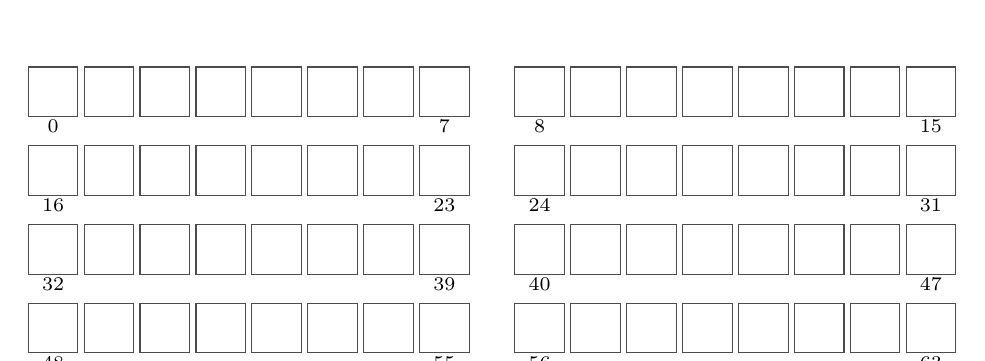
\begin{tikzpicture}
  \fsgrid{}{white}{0//fsW}
\end{tikzpicture}

{\small The disk as a plain array of 64 blocks (nothing assigned yet).}
\end{center}

\subsection{Similarity to memory?}

\textbf{Same principle:} map a logical abstraction to a physical resource
(here, process address spaces to memory frames; in a file system, files to
disk blocks).

\begin{center}
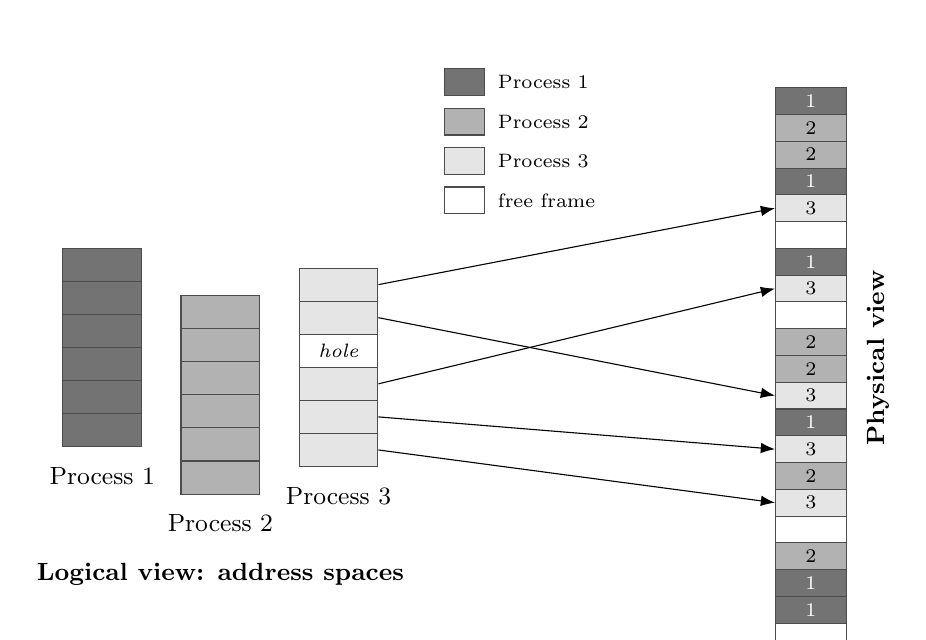
\begin{tikzpicture}[pg/.style={draw=black!70, minimum width=1.0cm,
                     minimum height=0.42cm, inner sep=0pt, font=\scriptsize},
                    fr/.style={draw=black!70, minimum width=0.9cm,
                     minimum height=0.34cm, inner sep=0pt, font=\scriptsize},
                    >={Latex[length=1.8mm]}]
  % process address spaces
  \foreach \k in {1,...,6} {
    \node[pg, fill=black!55] (a\k) at (0, -0.42*\k) {};
    \node[pg, fill=black!30] (b\k) at (1.5, -0.6-0.42*\k) {};
    \node[pg, fill=black!10] (c\k) at (3.0, -0.25-0.42*\k) {};
  }
  \node[pg, fill=white] at (c3) {\itshape hole};
  \node[font=\small] at (0,-3.1) {Process 1};
  \node[font=\small] at (1.5,-3.7) {Process 2};
  \node[font=\small] at (3.0,-3.35) {Process 3};
  \node[font=\small\bfseries] at (1.5,-4.35) {Logical view: address spaces};
  % physical memory
  \foreach \l [count=\k] in {1,2,2,1,3,,1,3,,2,2,3,1,3,2,3,,2,1,1,} {
    \ifnum\pdfstrcmp{\l}{1}=0 \node[fr, fill=black!55, text=white] (m\k) at (9, 2.0-0.34*\k) {1};\fi
    \ifnum\pdfstrcmp{\l}{2}=0 \node[fr, fill=black!30] (m\k) at (9, 2.0-0.34*\k) {2};\fi
    \ifnum\pdfstrcmp{\l}{3}=0 \node[fr, fill=black!10] (m\k) at (9, 2.0-0.34*\k) {3};\fi
    \ifnum\pdfstrcmp{\l}{}=0  \node[fr, fill=white] (m\k) at (9, 2.0-0.34*\k) {};\fi
  }
  \node[font=\small\bfseries, rotate=90] at (9.85,-1.6) {Physical view};
  % legend
  \foreach \f/\t/\c/\y in {black!55/Process 1/white/1.9, black!30/Process 2/black/1.4,
                            black!10/Process 3/black/0.9, white/free frame/white/0.4} {
    \node[fr, fill=\f, minimum width=0.5cm] at (4.6,\y) {};
    \node[font=\scriptsize, anchor=west] at (4.9,\y) {\t};
  }
  % process 3 mappings
  \draw[->] (c1.east) -- (m5.west);
  \draw[->] (c2.east) -- (m12.west);
  \draw[->] (c4.east) -- (m8.west);
  \draw[->] (c5.east) -- (m14.west);
  \draw[->] (c6.east) -- (m16.west);
\end{tikzpicture}

{\small Process 3's pages map to scattered frames; its third page is a hole.}
\end{center}

% ===========================================================================
\section{Allocation strategies}\label{sec:alloc}
% ===========================================================================

There are many different approaches to deciding which disk blocks hold a
file's data:
\begin{itemize}
  \item Contiguous
  \item Extent-based
  \item Linked
  \item File-allocation Tables
  \item Indexed
  \item Multi-level Indexed
\end{itemize}

\begin{keybox}[Questions used to evaluate every strategy]
\begin{enumerate}
  \item Amount of \textbf{fragmentation} (internal and external): free space
        that can't be used.
  \item Ability to \textbf{grow} a file over time?
  \item Performance of \textbf{sequential accesses} (contiguous layout)?
  \item Speed to find data blocks for \textbf{random accesses}?
  \item Wasted space for \textbf{meta-data overhead} (everything that isn't
        data)? Meta-data must be stored persistently too!
\end{enumerate}
\end{keybox}


The running example uses four files \textbf{A}, \textbf{B}, \textbf{C},
\textbf{D}; white blocks are free.

\keepspace{8\baselineskip}
\subsection{Contiguous allocation}

\begin{itemize}
  \item Allocate each file to \textbf{contiguous} sectors on disk.
  \begin{itemize}
    \item \textbf{Meta-data:} starting block and size of file.
    \item The OS allocates by finding sufficient free space.
    \begin{itemize}
      \item Must predict the future size of the file. Should space be
            reserved?
    \end{itemize}
    \item Example: IBM OS/360.
  \end{itemize}
\end{itemize}

\begin{center}
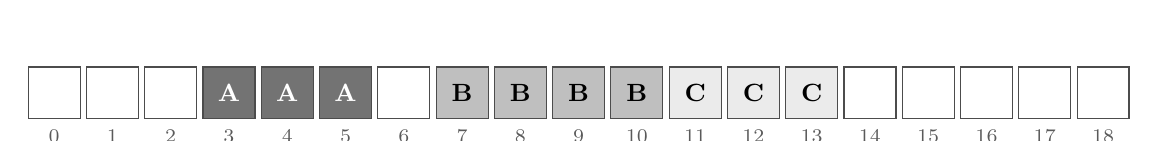
\begin{tikzpicture}
  \allocstrip{e,e,e,A,A,A,e,B,B,B,B,C,C,C,e,e,e,e,e}{0}
  \stripindex{19}{-0.55}
\end{tikzpicture}

{\small A = blocks 3--5 (start 3, size 3); B = 7--10 (start 7, size 4);
C = 11--13 (start 11, size 3). Free: 0--2, 6, 14--18.}
\end{center}

\begin{center}
\renewcommand{\arraystretch}{1.2}
\begin{tabularx}{\textwidth}{@{}lX@{}}
  \toprule
  \textbf{Question} & \textbf{Contiguous allocation} \\
  \midrule
  Fragmentation (internal and external)? & $-$ Horrible external frag (needs periodic compaction) \\
  Ability to grow file over time? & $-$ May not be able to grow without moving \\
  Seek cost for sequential accesses? & $+$ Excellent performance \\
  Speed to calculate random accesses? & $+$ Simple calculation \\
  Wasted space for meta-data? & $+$ Little overhead for meta-data \\
  \bottomrule
\end{tabularx}

{\small (The slide's grow answer reads ``May not be able to without moving'';
the missing word is ``grow''.)}
\end{center}


\keepspace{8\baselineskip}
\subsection{Small number of extents}

\begin{itemize}
  \item Allocate multiple contiguous regions (\textbf{extents}) per file.
  \begin{itemize}
    \item \textbf{Meta-data:} a small array (2--6) designating each extent.
          Each entry: starting block and size.
  \end{itemize}
\end{itemize}

\begin{center}
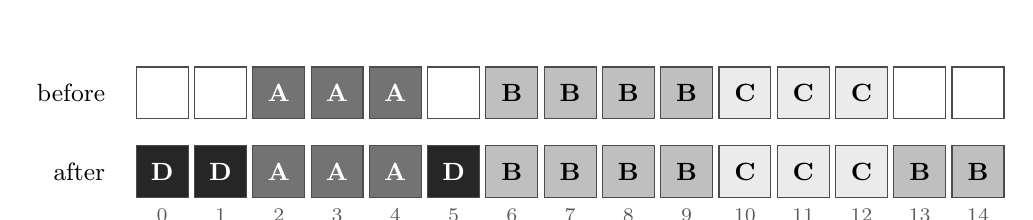
\begin{tikzpicture}
  \node[font=\small, anchor=east] at (-0.6,0) {before};
  \allocstrip{e,e,A,A,A,e,B,B,B,B,C,C,C,e,e}{0}
  \node[font=\small, anchor=east] at (-0.6,-1.0) {after};
  \allocstrip{D,D,A,A,A,D,B,B,B,B,C,C,C,B,B}{-1.0}
  \stripindex{15}{-1.55}
\end{tikzpicture}

{\small New file D uses the holes: extents (0, 2) and (5, 1). File B grows by
a second extent (13, 2), so B = \{(6, 4), (13, 2)\}. A = \{(2, 3)\},
C = \{(10, 3)\}. Each extent is written as (start, size).}
\end{center}

\begin{center}
\renewcommand{\arraystretch}{1.2}
\begin{tabularx}{\textwidth}{@{}lX@{}}
  \toprule
  \textbf{Question} & \textbf{Small number of extents} \\
  \midrule
  Fragmentation (internal and external)? & $-$ Helps external fragmentation \\
  Ability to grow file over time? & $-$ Can grow (until run out of extents) \\
  Seek cost for sequential accesses? & $+$ Still good performance \\
  Speed to calculate random accesses? & $+$ Still simple calculation \\
  Wasted space for meta-data? & $+$ Still small overhead for meta-data \\
  \bottomrule
\end{tabularx}
\end{center}

(``Helps'' external fragmentation is marked $-$ because it is only a partial
fix: each extent still needs a contiguous hole.)

\keepspace{8\baselineskip}
\subsection{Linked allocation}\label{sec:linked}

\begin{itemize}
  \item Allocate a linked list of \textbf{fixed-sized} blocks (multiple
        sectors).
  \begin{itemize}
    \item \textbf{Meta-data:} location of the first block of the file. Each
          block also contains a pointer to the next block.
    \item Examples: TOPS-10, Alto.
  \end{itemize}
\end{itemize}

\begin{center}
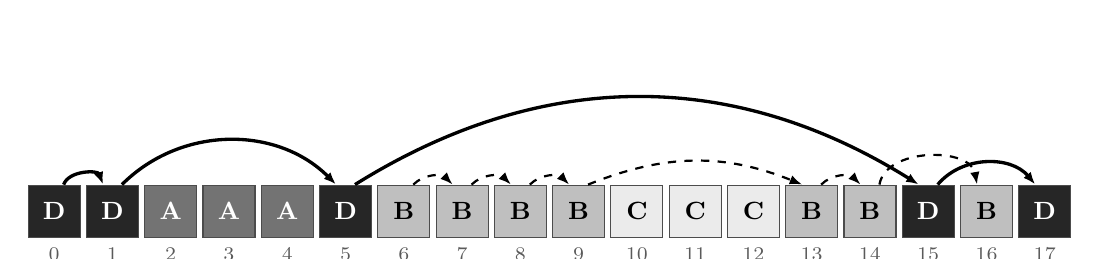
\begin{tikzpicture}[>={Latex[length=1.6mm]}]
  \allocstrip{D,D,A,A,A,D,B,B,B,B,C,C,C,B,B,D,B,D}{0}
  % file D: pointers drawn above
  \foreach \a/\b/\ang in {0/1/70, 1/5/45, 5/15/32, 15/17/50} {
    \draw[->, very thick] ([xshift=0.12cm]s\a.north) to[bend left=\ang] ([xshift=-0.12cm]s\b.north);
  }
  % file B: pointers drawn lower, dashed
  \foreach \a/\b/\ang in {6/7/45, 7/8/45, 8/9/45, 9/13/22, 13/14/45, 14/16/80} {
    \draw[->, thick, dashed] ([xshift=0.12cm]s\a.north) to[bend left=\ang] ([xshift=-0.12cm]s\b.north);
  }
  \stripindex{18}{-0.55}
\end{tikzpicture}

{\small File D (solid, taller arcs): 0 \(\to\) 1 \(\to\) 5 \(\to\) 15
\(\to\) 17 (end). File B (dashed, lower arcs): 6 \(\to\) 7 \(\to\) 8
\(\to\) 9 \(\to\) 13 \(\to\) 14 \(\to\) 16 (end). A (2--4) and C (10--12)
are chained the same way; their arrows are not drawn.}
\end{center}

\begin{center}
\renewcommand{\arraystretch}{1.2}
\begin{tabularx}{\textwidth}{@{}lX@{}}
  \toprule
  \textbf{Question} & \textbf{Linked allocation} \\
  \midrule
  Fragmentation (internal and external)? & $+$ No external frag (use any block); internal? \\
  Ability to grow file over time? & $+$ Can grow easily \\
  Seek cost for sequential accesses? & $\pm$ Depends on data layout \\
  Speed to calculate random accesses? & $-$ Ridiculously poor \\
  Wasted space for meta-data? & $-$ Waste pointer per block \\
  \bottomrule
\end{tabularx}
\end{center}


\begin{quizbox}[Trade-off: block size (it does not need to equal the sector size). Larger \(\to\) ?? Smaller \(\to\) ??]
\textbf{Larger:} less pointer overhead and fewer seeks, but more internal
fragmentation. \textbf{Smaller:} less internal fragmentation, but more
pointers and worse performance.
\end{quizbox}

\keepspace{8\baselineskip}
\subsection{File-Allocation Table (FAT)}

\begin{itemize}
  \item A variation of linked allocation.
  \begin{itemize}
    \item Keep the linked-list information for all files in an
          \textbf{on-disk FAT table} (instead of inside the data blocks).
    \item \textbf{Meta-data:} location of the first block of the file, and
          the FAT table itself.
  \end{itemize}
\end{itemize}

\begin{quizbox}[Draw the corresponding FAT table?]
One entry per disk block: entry \(b\) holds the next block of \(b\)'s file
(``end'' for the last). For the linked-allocation example:

\smallskip
\begin{center}
\footnotesize
\setlength{\tabcolsep}{2.6pt}
\renewcommand{\arraystretch}{1.25}
\begin{tabular}{@{}l*{18}{c}@{}}
  \toprule
  \textbf{block} & 0 & 1 & 2 & 3 & 4 & 5 & 6 & 7 & 8 & 9 & 10 & 11 & 12 & 13 & 14 & 15 & 16 & 17 \\
  \textbf{file}  & D & D & A & A & A & D & B & B & B & B & C & C & C & B & B & D & B & D \\
  \midrule
  \textbf{next}  & 1 & 5 & 3 & 4 & end & 15 & 7 & 8 & 9 & 13 & 11 & 12 & end & 14 & 16 & 17 & end & end \\
  \bottomrule
\end{tabular}
\end{center}

\smallskip
First blocks: A \(\to\) 2, B \(\to\) 6, C \(\to\) 10, D \(\to\) 0. (The
``file'' row is only for reading; it is not stored.)
\end{quizbox}

\noindent\textbf{Comparison to linked allocation:}
\begin{itemize}
  \item Same basic advantages and disadvantages.
  \item \textbf{Disadvantage:} read from \emph{two} disk locations for every
        data read (the FAT entry and the data block).
  \item \textbf{Optimization:} cache the FAT in main memory.
  \begin{itemize}
    \item \textbf{Advantage:} greatly improves random accesses (the chain
          is followed in memory).
    \item \textbf{What portions should be cached? Scale with larger file
          systems?} The FAT grows with the disk (one entry per block), so
          for large disks only part of it (e.g.\ files in use) can be
          cached.
  \end{itemize}
\end{itemize}

\keepspace{8\baselineskip}
\subsection{Indexed allocation}

\begin{itemize}
  \item Allocate fixed-sized blocks for each file.
  \begin{itemize}
    \item \textbf{Meta-data:} a fixed-sized array of block pointers.
    \item Allocate space for the pointers at file creation time.
  \end{itemize}
\end{itemize}

\begin{center}
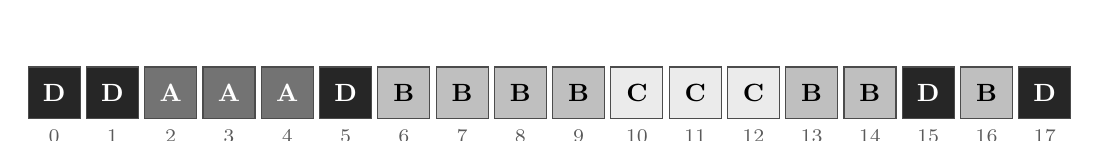
\begin{tikzpicture}
  \allocstrip{D,D,A,A,A,D,B,B,B,B,C,C,C,B,B,D,B,D}{0}
  \stripindex{18}{-0.55}
\end{tikzpicture}

\end{center}

\keepspace{9\baselineskip}
\begin{itemize}
  \item \textbf{Advantages}
  \begin{itemize}
    \item No external fragmentation.
    \item Files can be easily grown up to max file size.
    \item Supports random access.
  \end{itemize}
  \item \textbf{Disadvantages}
  \begin{itemize}
    \item Large overhead for meta-data: wastes space for unneeded pointers
          (most files are small!).
  \end{itemize}
\end{itemize}

\keepspace{8\baselineskip}
\subsection{Multi-level indexing}\label{sec:multilevel}

\begin{itemize}
  \item A variation of indexed allocation.
  \begin{itemize}
    \item Dynamically allocate a hierarchy of pointers to blocks \emph{as
          needed}.
    \item \textbf{Meta-data:} a small number of pointers allocated
          statically, plus additional pointers to blocks of pointers.
    \item Examples: UNIX FFS-based file systems, ext2, ext3.
  \end{itemize}
\end{itemize}

\begin{center}
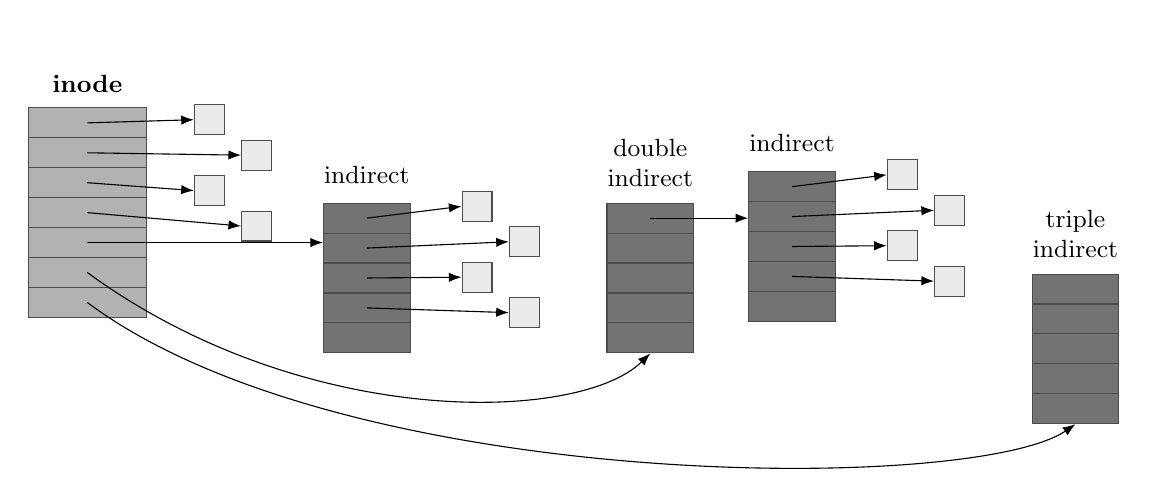
\begin{tikzpicture}[>={Latex[length=1.6mm]},
    sl/.style={draw=black!70, fill=black!30, minimum width=1.5cm,
               minimum height=0.38cm, inner sep=0pt},
    isl/.style={draw=black!70, fill=black!55, minimum width=1.1cm,
                minimum height=0.38cm, inner sep=0pt},
    dat/.style={draw=black!70, fill=black!8, minimum size=0.38cm, inner sep=0pt}]
  % inode: 7 slots (4 direct, then single, double, triple)
  \foreach \k in {0,...,6} { \node[sl] (n\k) at (0.75, -0.19-\k*0.38) {}; }
  \node[font=\small\bfseries] at (0.75,0.3) {inode};
  % direct data blocks
  \node[dat] (d0) at (2.3,-0.15) {};
  \node[dat] (d1) at (2.9,-0.6) {};
  \node[dat] (d2) at (2.3,-1.05) {};
  \node[dat] (d3) at (2.9,-1.5) {};
  \foreach \k in {0,...,3} { \draw[->] (n\k.center) -- (d\k.west); }
  % single indirect
  \foreach \k in {0,...,4} { \node[isl] (s\k) at (4.3, -1.4-\k*0.38) {}; }
  \node[font=\small, align=center] at (4.3,-0.85) {indirect};
  \draw[->] (n4.center) -- (n4.center -| s2.west);
  \node[dat] (e0) at (5.7,-1.25) {};
  \node[dat] (e1) at (6.3,-1.7) {};
  \node[dat] (e2) at (5.7,-2.15) {};
  \node[dat] (e3) at (6.3,-2.6) {};
  \foreach \k in {0,...,3} { \draw[->] (s\k.center) -- (e\k.west); }
  % double indirect
  \foreach \k in {0,...,4} { \node[isl] (t\k) at (7.9, -1.4-\k*0.38) {}; }
  \node[font=\small, align=center] at (7.9,-0.7) {double\\indirect};
  \draw[->] (n5.center) .. controls (3.5,-4.1) and (7.0,-4.0) .. (t4.south);
  % indirect below double
  \foreach \k in {0,...,4} { \node[isl] (u\k) at (9.7, -1.0-\k*0.38) {}; }
  \node[font=\small, align=center] at (9.7,-0.45) {indirect};
  \draw[->] (t0.center) -- (t0.center -| u1.west);
  \node[dat] (f0) at (11.1,-0.85) {};
  \node[dat] (f1) at (11.7,-1.3) {};
  \node[dat] (f2) at (11.1,-1.75) {};
  \node[dat] (f3) at (11.7,-2.2) {};
  \foreach \k in {0,...,3} { \draw[->] (u\k.center) -- (f\k.west); }
  % triple indirect
  \foreach \k in {0,...,4} { \node[isl] (w\k) at (13.3, -2.3-\k*0.38) {}; }
  \node[font=\small, align=center] at (13.3,-1.6) {triple\\indirect};
  \draw[->] (n6.center) .. controls (4.0,-4.9) and (12.0,-4.9) .. (w4.south);
\end{tikzpicture}

{\small The inode has a few \emph{direct} pointers (top four slots) to data
blocks, then a pointer to a single \emph{indirect} block (a block of
pointers to data blocks), a pointer to a \emph{double indirect} block
(pointers to indirect blocks), and a pointer to a \emph{triple indirect}
block (pointers to double indirect blocks).}
\end{center}

\noindent\textbf{Comparison to indexed allocation:}
\begin{itemize}
  \item \textbf{Advantage:} does not waste space for unneeded pointers.
  \begin{itemize}
    \item Still fast access for small files.
    \item Can grow to what size?? (answered below)
  \end{itemize}
  \item \textbf{Disadvantage:} need to read indirect blocks of pointers to
        calculate addresses (extra disk read).
  \begin{itemize}
    \item Keep indirect blocks cached in main memory.
  \end{itemize}
\end{itemize}

\keepspace{14\baselineskip}
\begin{solbox}[Can grow to what size??]
\textbf{General formula.} Let \(D\) be the number of direct pointers in the
inode, \(B\) the block size, and \(P = B/(\text{pointer size})\) the number of
pointers that fit in one block. A single indirect block reaches \(P\) data
blocks, a double indirect block \(P^2\), and a triple indirect block \(P^3\):
\[
\text{max file size} = (D + P + P^2 + P^3)\times B .
\]

\textbf{For the slide's figure} (\(D = 4\) direct pointers, plus one single,
one double and one triple indirect pointer), using the 4~KB block size
(``Assume each block is 4KB'') and the 4-byte pointers (``Assume 4-byte
addrs'') given later in the lecture, \(P = 4096/4 = 1024\):
\[
(4 + 1024 + 1024^2 + 1024^3)\times 4\,\text{KB}
= 1\,074\,791\,428 \times 4\,\text{KB} \approx 4\,\text{TB}.
\]
(16 KB direct + 4 MB single + 4 GB double + 4 TB triple: the triple-indirect
term dominates.)
\end{solbox}
\noindent{\small (Not from the slides: real UNIX/ext2 inodes have 12 direct pointers
instead of 4, which changes the total only by 32~KB.)}

\keepspace{8\baselineskip}
\subsection{Flexible number of extents}

\begin{itemize}
  \item Modern file systems: \textbf{dynamic} multiple contiguous regions
        (extents) per file.
  \begin{itemize}
    \item Organize the extents into a \textbf{multi-level tree} structure.
    \begin{itemize}
      \item Each leaf node: starting block and contiguous size.
      \item Minimizes meta-data overhead when a file has few extents.
      \item Allows growth beyond a fixed number of extents.
    \end{itemize}
  \end{itemize}
\end{itemize}

\begin{center}
\renewcommand{\arraystretch}{1.2}
\begin{tabularx}{\textwidth}{@{}lX@{}}
  \toprule
  \textbf{Question} & \textbf{Flexible number of extents} \\
  \midrule
  Fragmentation (internal and external)? & $+$ Both reasonable \\
  Ability to grow file over time? & $+$ Can grow \\
  Seek cost for sequential accesses? & $+$ Still good performance \\
  Speed to calculate random accesses? & $\pm$ Some calculations depending on size \\
  Wasted space for meta-data? & $+$ Relatively small overhead \\
  \bottomrule
\end{tabularx}
\end{center}

% ===========================================================================
\section{The on-disk structures of a simple file system}\label{sec:vsfs}
% ===========================================================================

\textbf{Assume multi-level indexing.} It is a simple approach, and more
complex file systems build from these basic data structures. The on-disk
structures we will need are:
\begin{itemize}
  \item data block
  \item inode table
  \item indirect block
  \item directories
  \item data bitmap
  \item inode bitmap
  \item superblock
\end{itemize}
The slides build the layout of the 64-block disk step by step, starting
from the empty disk. \textbf{Assume each block is 4~KB.}

\keepspace{8\baselineskip}
\subsection{Data blocks}

Blocks \textbf{8--63} become the \textbf{data region} (marked D).

\begin{center}
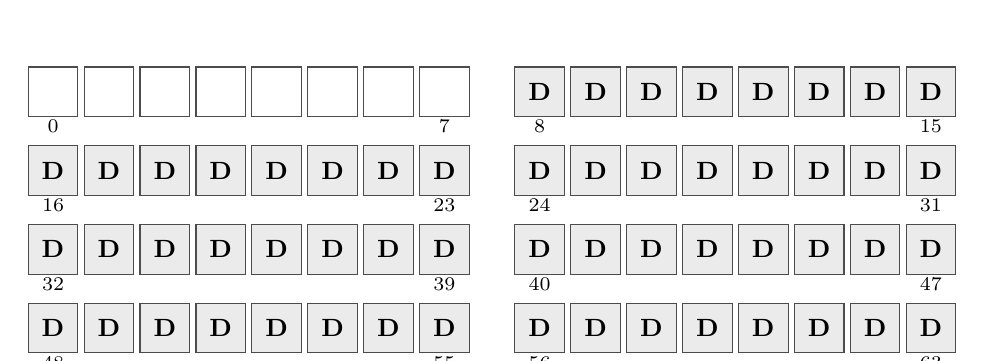
\begin{tikzpicture}
  \fsgrid{D}{black!8}{0//fsW}
\end{tikzpicture}

{\small Data region: blocks 8--63.}
\end{center}

\keepspace{8\baselineskip}
\subsection{Inodes and the inode table}

The \textbf{inode table} (the array of inodes) occupies blocks \textbf{3--7}
(marked I).

\begin{center}
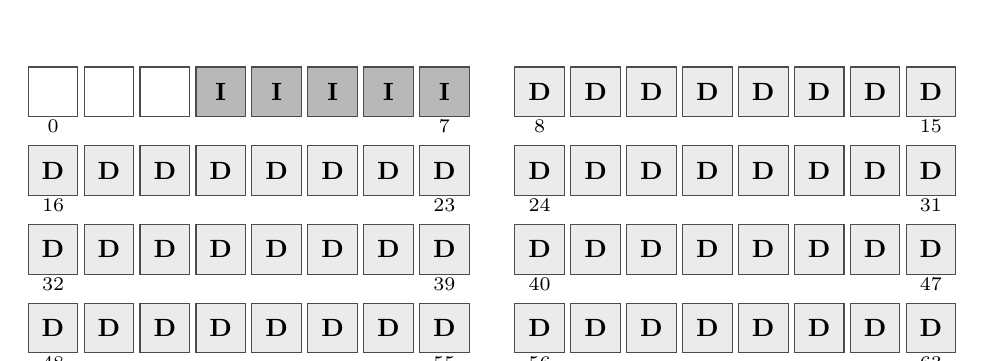
\begin{tikzpicture}
  \fsgrid{D}{black!8}{3/I/fsI,4/I/fsI,5/I/fsI,6/I/fsI,7/I/fsI}
\end{tikzpicture}

{\small Inode table: blocks 3--7. Data: blocks 8--63.}
\end{center}

\keepspace{8\baselineskip}
\subsection{One inode block}

\begin{itemize}
  \item Each inode is typically 256 bytes (depends on the FS, maybe 128
        bytes).
  \item A disk block is 4~KB.
  \item So there are \(4096/256 = \mathbf{16}\) \textbf{inodes per inode
        block}.
\end{itemize}

\begin{center}
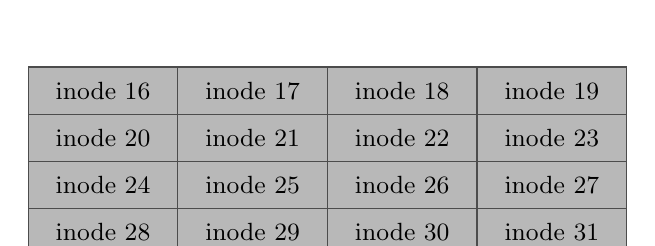
\begin{tikzpicture}[ic/.style={draw=black!70, fill=black!28, minimum width=1.9cm,
                    minimum height=0.6cm, font=\small}]
  \foreach \r in {0,...,3} {
    \foreach \c in {0,...,3} {
      \pgfmathtruncatemacro{\n}{16+4*\r+\c}
      \node[ic] at (\c*1.9, -\r*0.6) {inode \n};
    }
  }
\end{tikzpicture}

{\small One 4~KB inode block: 16 inodes of 256 bytes (here inodes 16--31).}
\end{center}


\keepspace{14\baselineskip}
\subsection{The inode}


\begin{lstlisting}[language={}, numbers=none]
type          (file or dir?)
uid           (owner)
rwx           (permissions)
size          (in bytes)
Blocks
time          (access)
ctime         (create)
links_count   (# paths)
addrs[N]      (N data blocks)
\end{lstlisting}

{\small (\texttt{ctime} is labelled ``create'' on the slide; in real Unix it is
the inode \emph{change} time.)}

\keepspace{8\baselineskip}
\subsection{Inodes point to data blocks}

Inodes point (through \texttt{addrs[]}) to blocks in the data region.

\begin{center}
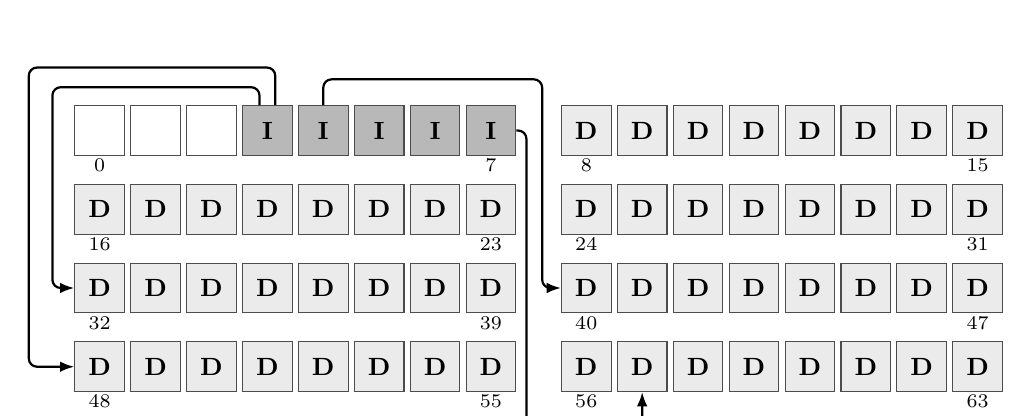
\begin{tikzpicture}[>={Latex[length=1.8mm]}]
  \fsgrid{D}{black!8}{3/I/fsI,4/I/fsI,5/I/fsI,6/I/fsI,7/I/fsI}
  \begin{scope}[thick, rounded corners=3pt]
    \draw[->] ([xshift=-0.1cm]b3.north) |- (-0.6,0.55) |- (b32.west);
    \draw[->] ([xshift=0.1cm]b3.north) |- (-0.9,0.8) |- (b48.west);
    \draw[->] (b4.north) |- (5.62,0.65) |- (b40.west);
    \draw[->] (b7.east) -- (5.42,0) |- (6.89,-3.75) -- (b57.south);
  \end{scope}
\end{tikzpicture}

{\small Inodes in block 3 point to blocks 32 and 48; block 4 to 40; block 7 to 57.}
\end{center}

\keepspace{8\baselineskip}
\subsection{Max file size with only direct pointers}

\begin{center}
\begin{minipage}[t]{0.25\textwidth}
\begin{lstlisting}[language={}, numbers=none]
type
uid
rwx
size
blocks
time
ctime
links_count
addrs[N]
\end{lstlisting}
\end{minipage}\hfill
\begin{minipage}[t]{0.68\textwidth}
\begin{itemize}
  \item Assume single level (just pointers to data blocks).
  \item \textbf{What is the max file size?}
  \item Assume 256-byte inodes (all can be used for pointers).
  \item Assume 4-byte addrs.
  \item \textbf{How to get larger files?}
\end{itemize}
\end{minipage}
\end{center}

\begin{solbox}[What is the max file size? (single level: direct pointers only)]
\(256 / 4 = 64\) pointers, each to a 4~KB block:
\(64 \times 4\,\text{KB} = \mathbf{256\,KB}\)! (This is for direct pointers
only; indirect blocks allow much larger files.)
\end{solbox}

\begin{quizbox}[How to get larger files?]
Use \textbf{indirect blocks}: inode pointers to blocks of pointers (next
section).
\end{quizbox}

\keepspace{8\baselineskip}
% ===========================================================================
\section{Direct and indirect pointers}\label{sec:indirect}
% ===========================================================================

\keepspace{12\baselineskip}
\subsection{Direct pointers only}

Every address in the inode points directly to a data block:

\begin{center}
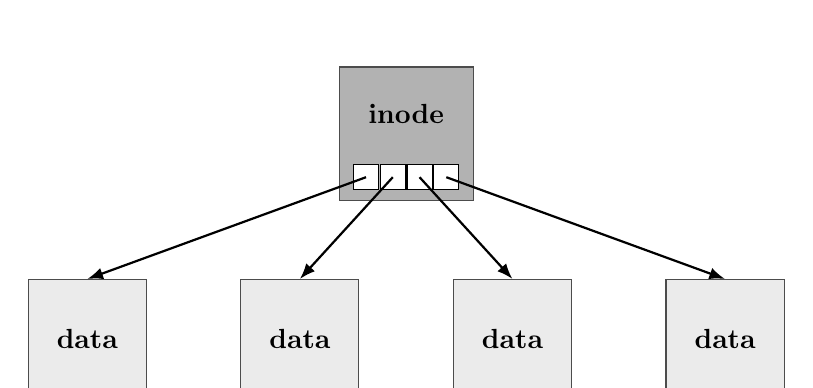
\begin{tikzpicture}
  \inodetree{data,data,data,data}
\end{tikzpicture}
\end{center}

\keepspace{8\baselineskip}
\subsection{Indirect blocks}

Every inode pointer points to an \textbf{indirect block}, a block of pointers
to data blocks.

\begin{center}
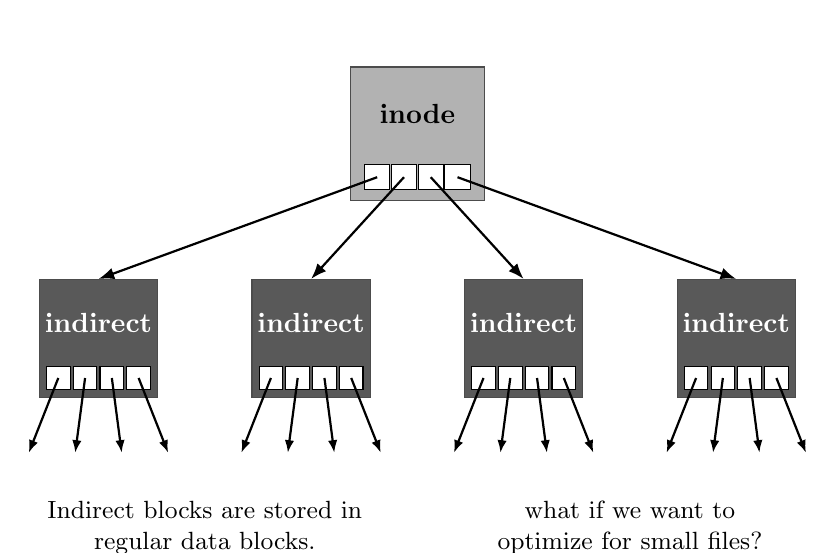
\begin{tikzpicture}
  \inodetree{indirect,indirect,indirect,indirect}
  \node[font=\small, align=center] at (-2.7,-5.0) {Indirect blocks are stored in\\regular data blocks.};
  \node[font=\small, align=center] at (2.7,-5.0) {what if we want to\\optimize for small files?};
\end{tikzpicture}
\end{center}

Indirect blocks are allocated from the data region. But now every file, even
a tiny one, needs an extra indirect block and disk read.

\keepspace{8\baselineskip}
\subsection{Better for small files}

\begin{quizbox}[What if we want to optimize for small files?]
Mix the two: keep the first pointers \textbf{direct} and make only the
last one \textbf{indirect}.
\end{quizbox}

\begin{center}
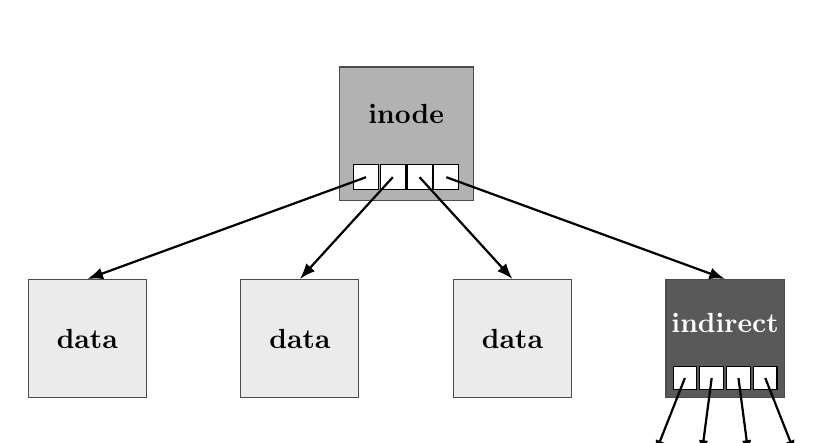
\begin{tikzpicture}
  \inodetree{data,data,data,indirect}
\end{tikzpicture}
\end{center}
\noindent\textbf{Better for small files:} small files use only the direct
pointers (no extra read); large files grow through the indirect block.


% ===========================================================================
\section{Finding an inode on disk}\label{sec:inodeoffset}
% ===========================================================================

Given the inode number, the file system computes where the inode is. The
inode table is in blocks 3--7:

\begin{center}
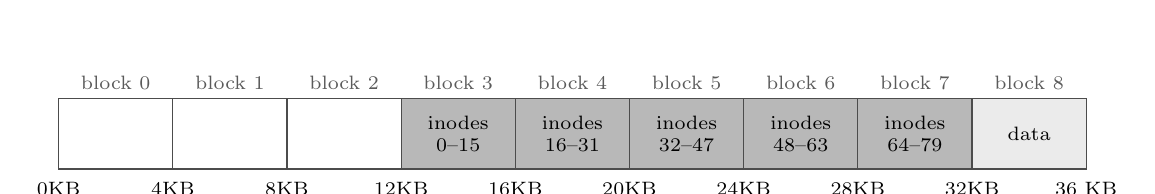
\begin{tikzpicture}[zb/.style={draw=black!70, minimum width=1.45cm,
                    minimum height=0.9cm, inner sep=1pt, font=\scriptsize,
                    align=center}]
  \foreach \l/\f [count=\k from 0] in {{}/white,{}/white,{}/white,
      {inodes\\0--15}/black!28,{inodes\\16--31}/black!28,{inodes\\32--47}/black!28,
      {inodes\\48--63}/black!28,{inodes\\64--79}/black!28,{data}/black!8} {
    \node[zb, fill=\f] (z\k) at (\k*1.45, 0) {\l};
    \node[font=\scriptsize, text=g3] at (\k*1.45, 0.65) {block \k};
    \pgfmathtruncatemacro{\kb}{4*\k}
    \node[font=\scriptsize] at (\k*1.45-0.725, -0.7) {\kb KB};
  }
  \node[font=\scriptsize] at (8*1.45+0.725, -0.7) {36 KB};
\end{tikzpicture}

{\small The inode table starts at block 3, i.e.\ at byte address
\(3\times4\,\text{KB} = 12\,\text{KB} = 12288\).}
\end{center}

\begin{keybox}[How to locate inode number \(n\)]
With 256-byte inodes, 16 inodes per 4~KB block, and the inode table starting
at block 3:
\begin{align*}
  \text{block}            &= 3 + \lfloor n / 16 \rfloor, \\
  \text{offset in block}  &= (n \bmod 16)\times 256 \text{ bytes}, \\
  \text{byte address}     &= \text{block}\times4096 + \text{offset in block}
                           = 12288 + 256\,n.
\end{align*}

\end{keybox}

\begin{quizbox}[Assume 256-byte inodes (16 inodes/block). What is the offset for inode number 0?]
\(\lfloor 0/16\rfloor = 0\), \(0 \bmod 16 = 0\). Inode 0 is the first inode
of the first inode block: \textbf{block 3, offset 0} within it, i.e.\ byte
address \(3\times4096 + 0 = \mathbf{12288}\) (= 12~KB).
\end{quizbox}

\begin{quizbox}[What is the offset for inode number 4?]
\(\lfloor 4/16\rfloor = 0\), \(4 \bmod 16 = 4\). Still in \textbf{block 3},
at offset \(4\times256 = \mathbf{1024}\) bytes within the block, i.e.\
byte address \(12288 + 1024 = \mathbf{13312}\) (= 13~KB).
\end{quizbox}

\begin{quizbox}[What is the offset for inode number 40?]
\(40 = 2\times16 + 8\), so \(\lfloor 40/16\rfloor = 2\) and
\(40 \bmod 16 = 8\). Skip two full inode blocks (3 and 4): inode 40 is in
\textbf{block 5} (which holds inodes 32--47), at offset
\(8\times256 = \mathbf{2048}\) bytes within the block. Byte address:
\(5\times4096 + 2048 = \mathbf{22528}\) (= 22~KB).
\end{quizbox}

% ===========================================================================
\section{Directories}
% ===========================================================================

File systems vary. A \textbf{common design}:
\begin{itemize}
  \item Store \textbf{directory entries in data blocks}.
  \begin{itemize}
    \item Large directories just use multiple data blocks.
    \item Use a bit in the inode (the \texttt{type} field) to distinguish
          directories from files.
  \end{itemize}
  \item Various formats could be used: \textbf{lists}, \textbf{b-trees}.
\end{itemize}

\keepspace{8\baselineskip}
\subsection{Simple directory list example}

\begin{center}
\begin{minipage}[t]{0.38\textwidth}
\centering
\textbf{Directory on the slide}\\[0.1em]
{\footnotesize (inode numbers from the slide, not the 64-block toy FS)}\\[0.2em]
\renewcommand{\arraystretch}{1.2}
\begin{tabular}{@{}ccc@{}}
  \toprule
  \textbf{valid} & \textbf{name} & \textbf{inode} \\
  \midrule
  1 & \texttt{.}   & 134 \\
  1 & \texttt{..}  & 35 \\
  1 & \texttt{foo} & 80 \\
  1 & \texttt{bar} & 23 \\
  \bottomrule
\end{tabular}
\end{minipage}
\begin{minipage}[t]{0.38\textwidth}
\centering
\textbf{Answer: after} \texttt{unlink("foo")}\\[0.1em]
{\footnotesize (illustration, not on the slide)}\\[0.2em]
\renewcommand{\arraystretch}{1.2}
\begin{tabular}{@{}ccc@{}}
  \toprule
  \textbf{valid} & \textbf{name} & \textbf{inode} \\
  \midrule
  1 & \texttt{.}   & 134 \\
  1 & \texttt{..}  & 35 \\
  \textbf{0} & \texttt{foo} & 80 \\
  1 & \texttt{bar} & 23 \\
  \bottomrule
\end{tabular}
\end{minipage}
\end{center}


\begin{quizbox}[What does \texttt{unlink("foo")} do to this directory?]
The entry for \texttt{foo} is marked \textbf{invalid} (valid = 0), and
\texttt{links\_count} of inode 80 is decremented (freed at 0).
\end{quizbox}

\keepspace{8\baselineskip}
% ===========================================================================
\section{Free-space allocation: free lists vs.\ bitmaps}
% ===========================================================================

\textbf{How do we find free data blocks or free inodes?} Two options:
\begin{itemize}
  \item a \textbf{free list}: a linked list of the free blocks;
  \item \textbf{bitmaps}: one bit per block (or inode), 0 = free,
        1 = in use.
\end{itemize}

\keepspace{8\baselineskip}
\subsection{Free list: aging?}

\begin{quizbox}[What is the performance before/after aging?]
\begin{itemize}
  \item New FS: \textbf{good performance}.
  \item Few weeks old: \textbf{performance starts to degrade}.
\end{itemize}
\textbf{Problem:} the FS becomes fragmented over time. The free list makes
contiguous chunks hard to find.

\textbf{Hacky solutions:}
\begin{itemize}
  \item Occasional defrag of the disk.
  \item Keep the free list sorted.
\end{itemize}
{\small (The slide spells it ``Occassional''.)}
\end{quizbox}

\begin{center}
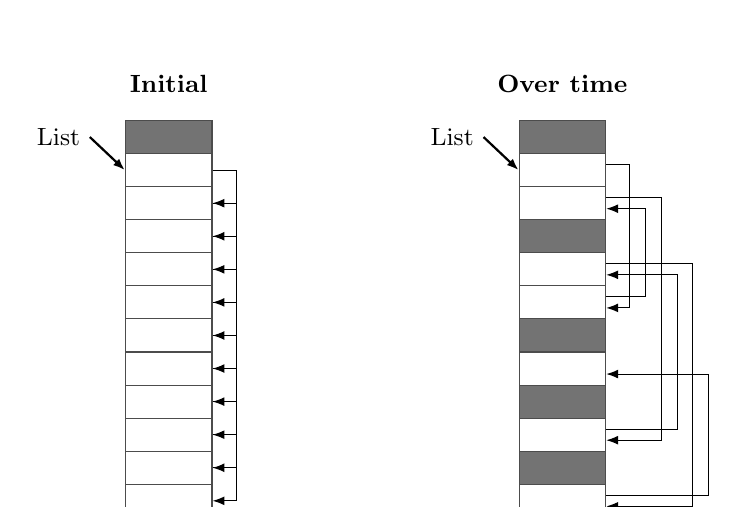
\begin{tikzpicture}[fc/.style={draw=black!70, minimum width=1.1cm,
                    minimum height=0.42cm, inner sep=0pt},
                    used/.style={fc, fill=black!55},
                    >={Latex[length=1.5mm]}]
  % initial
  \foreach \k in {1,...,12} { \node[fc] (L\k) at (0,-\k*0.42) {}; }
  \node[used] at (L1) {};
  \node[font=\small\bfseries] at (0,0.25) {Initial};
  \node[font=\small] (lh) at (-1.4,-0.42) {List};
  \draw[->, thick] (lh.east) -- (L2.west);
  \foreach \a/\b in {2/3,3/4,4/5,5/6,6/7,7/8,8/9,9/10,10/11,11/12} {
    \draw[->] (L\a.east) -- ++(0.3,0) |- (L\b.east);
  }
  % over time
  \foreach \k in {1,...,12} { \node[fc] (R\k) at (5,-\k*0.42) {}; }
  \foreach \k in {1,4,7,9,11} { \node[used] at (R\k) {}; }
  \node[font=\small\bfseries] at (5,0.25) {Over time};
  \node[font=\small] (rh) at (3.6,-0.42) {List};
  \draw[->, thick] (rh.east) -- (R2.west);
  \foreach \a/\b/\o in {2/6/0.3,6/3/0.5,3/10/0.7,10/5/0.9,5/12/1.1,12/8/1.3} {
    \draw[->] ([yshift=0.07cm]R\a.east) -- ++(\o,0) |- ([yshift=-0.07cm]R\b.east);
  }
\end{tikzpicture}

{\small Dark = in use. Initially the list is in disk order; over time it jumps
around the disk.}
\end{center}


\keepspace{8\baselineskip}
\subsection{Bitmaps?}\label{sec:bitmaps}

One bit per inode / data block (0 = free). The \textbf{inode bitmap} goes in
block 1 (i) and the \textbf{data bitmap} in block 2 (d):

\begin{center}
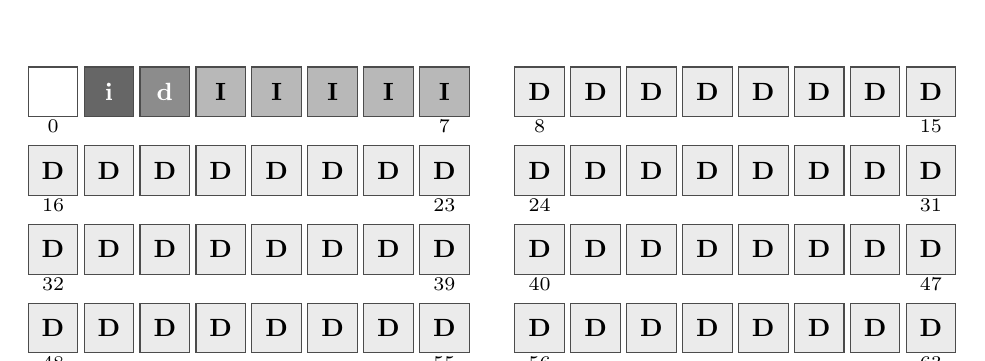
\begin{tikzpicture}
  \fsgrid{D}{black!8}{1/i/fsi,2/d/fsd,3/I/fsI,4/I/fsI,5/I/fsI,6/I/fsI,7/I/fsI}
\end{tikzpicture}

{\small Block 1: inode bitmap (i). Block 2: data bitmap (d). Block 0 is
still unassigned.}
\end{center}

Unlike a free list, the bitmap stays in disk order, so contiguous free runs
are easy to find.

\keepspace{8\baselineskip}
\subsection{Opportunity for inconsistency (fsck)}

(This slide is the first to show the bitmaps on disk, as in the grid above.)
The bitmaps duplicate information implied by the inodes and directories; a
crash in the middle of an update can leave them inconsistent.

\begin{defbox}[fsck (file system checker)]
A tool that scans the file system after a crash and repairs inconsistent
structures.
\end{defbox}

% ===========================================================================
\section{Superblock and the final layout}
% ===========================================================================

The file system needs to know basic FS \textbf{configuration meta-data}, like:
\begin{itemize}
  \item block size,
  \item number of inodes.
\end{itemize}
\keepspace{8\baselineskip}
\noindent\textbf{Store this in the superblock}, in block \textbf{0} (S):

\begin{center}
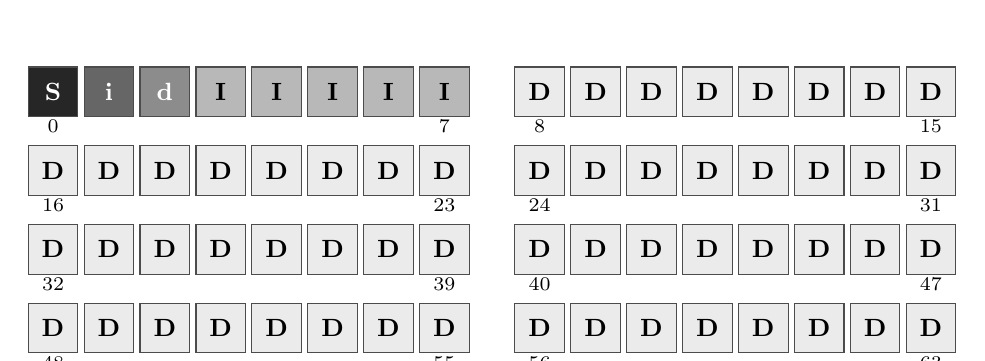
\begin{tikzpicture}
  \fsgrid{D}{black!8}{0/S/fsS,1/i/fsi,2/d/fsd,3/I/fsI,4/I/fsI,5/I/fsI,6/I/fsI,7/I/fsI}
\end{tikzpicture}

{\small The complete layout: S (block 0), inode bitmap i (1), data bitmap
d (2), inode table I (3--7), data D (8--63).}
\end{center}

\keepspace{8\baselineskip}
\subsection{Summary of the on-disk structures}

\begin{center}
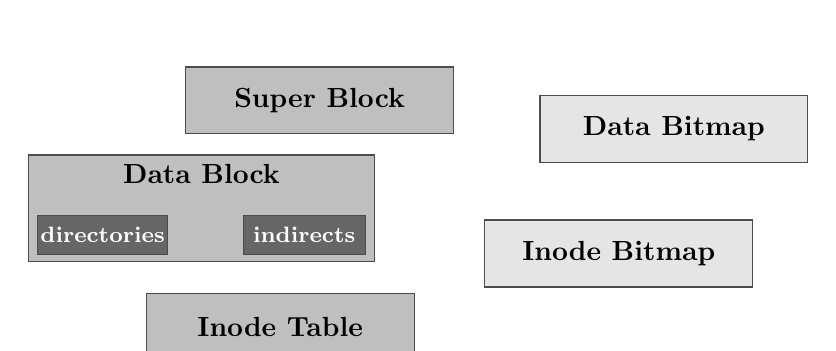
\begin{tikzpicture}[yscale=0.72, bx/.style={draw=black!70, fill=black!25, minimum width=3.4cm,
                    minimum height=0.85cm, font=\bfseries},
                    bm/.style={draw=black!70, fill=black!10, minimum width=3.4cm,
                    minimum height=0.85cm, font=\bfseries},
                    sm/.style={draw=black!70, fill=black!60, text=white,
                    minimum width=1.55cm, minimum height=0.5cm, inner sep=1pt,
                    font=\footnotesize\bfseries}]
  \node[bx] at (1.5,0) {Super Block};
  \node[bm] at (6.0,-0.5) {Data Bitmap};
  \node[bx, minimum width=4.4cm, minimum height=1.35cm] (db) at (0,-1.9) {};
  \node[font=\bfseries] at ([yshift=-0.35cm]db.north) {Data Block};
  \node[sm, anchor=south west] at ([xshift=0.12cm, yshift=0.12cm]db.south west) {directories};
  \node[sm, anchor=south east] at ([xshift=-0.12cm, yshift=0.12cm]db.south east) {indirects};
  \node[bm] at (5.3,-2.7) {Inode Bitmap};
  \node[bx] at (1.0,-4.0) {Inode Table};
\end{tikzpicture}

{\small Directories and indirect blocks are not separate regions: they live
inside data blocks.}
\end{center}

% ===========================================================================
\section{Part 2: Operations}
% ===========================================================================

Disk I/O for \textbf{create file}, \textbf{write}, \textbf{open}, \textbf{read},
\textbf{close} on \texttt{/foo/bar} (nothing cached; rows are in time order).

\begin{warnbox}[Two facts used in every trace]
\begin{itemize}
  \item Path traversal starts at the root inode (a well-known number).
  \item The disk reads and writes whole blocks, so updating one inode or bitmap
        bit means read the block, modify, write it back.
\end{itemize}
\end{warnbox}

\keepspace{22\baselineskip}
\subsection{create /foo/bar}

\begin{quizbox}[What needs to be read and written?]
\begin{center}
\small
\setlength{\tabcolsep}{3.5pt}
\renewcommand{\arraystretch}{1.18}
\begin{tabularx}{\linewidth}{@{}c*{7}{c}X@{}}
  \toprule
  & \multicolumn{2}{c}{\textbf{bitmap}} & \multicolumn{3}{c}{\textbf{inode}} & \multicolumn{2}{c}{\textbf{data}} & \\
  \cmidrule(lr){2-3}\cmidrule(lr){4-6}\cmidrule(lr){7-8}
  \textbf{\#} & data & inode & root & foo & bar & root & foo & \textbf{why} \\
  \midrule
  1  &  &  & read &  &  &  &  & find root's data blocks \\
  2  &  &  &  &  &  & read &  & look up \texttt{foo} \(\to\) its inode number \\
  3  &  &  &  & read &  &  &  & find \texttt{foo}'s data blocks \\
  4  &  &  &  &  &  &  & read & check \texttt{bar} does not exist; find a free slot \\
  5  &  & read &  &  &  &  &  & find a free inode \\
  6  &  & \textbf{write} &  &  &  &  &  & mark it allocated \\
  7  &  &  &  &  &  &  & \textbf{write} & add entry (\texttt{bar}, inode number) \\
  8  &  &  &  &  & read &  &  & read the block holding the new inode \\
  9  &  &  &  &  & \textbf{write} &  &  & initialize \texttt{bar}'s inode \\
  10 &  &  &  & \textbf{write} &  &  &  & update \texttt{foo}'s inode (size, times) \\
  \bottomrule
\end{tabularx}
\end{center}

\noindent\textbf{Total: 6 reads and 4 writes} (10 I/Os) to create one empty file.
\end{quizbox}


\begin{keybox}[Make directory]
Like create, plus: allocate a data block (data bitmap) holding the
``\texttt{.}'' and ``\texttt{..}'' entries; the new directory starts with
\texttt{links\_count} 2, and the parent's count goes up by 1.
\end{keybox}

\keepspace{8\baselineskip}
\subsection{open /foo/bar}

\begin{center}
\small
\setlength{\tabcolsep}{3.5pt}
\renewcommand{\arraystretch}{1.18}
\begin{tabularx}{\linewidth}{@{}c*{8}{c}X@{}}
  \toprule
  & \multicolumn{2}{c}{\textbf{bitmap}} & \multicolumn{3}{c}{\textbf{inode}} & \multicolumn{3}{c}{\textbf{data}} & \\
  \cmidrule(lr){2-3}\cmidrule(lr){4-6}\cmidrule(lr){7-9}
  \textbf{\#} & data & inode & root & foo & bar & root & foo & bar & \textbf{why} \\
  \midrule
  1 &  &  & read &  &  &  &  &  & find root's data blocks \\
  2 &  &  &  &  &  & read &  &  & look up \texttt{foo} \\
  3 &  &  &  & read &  &  &  &  & find \texttt{foo}'s data blocks \\
  4 &  &  &  &  &  &  & read &  & look up \texttt{bar} \\
  5 &  &  &  &  & read &  &  &  & bring \texttt{bar}'s inode into memory \\
  \bottomrule
\end{tabularx}
\end{center}

\noindent\textbf{Total: 5 reads, no writes}: just the path walk, ending with
\texttt{bar}'s inode in memory.

\keepspace{8\baselineskip}
\subsection{write to /foo/bar (assume the file exists and has been opened)}

\begin{center}
\small
\setlength{\tabcolsep}{3.5pt}
\renewcommand{\arraystretch}{1.18}
\begin{tabularx}{\linewidth}{@{}c*{8}{c}X@{}}
  \toprule
  & \multicolumn{2}{c}{\textbf{bitmap}} & \multicolumn{3}{c}{\textbf{inode}} & \multicolumn{3}{c}{\textbf{data}} & \\
  \cmidrule(lr){2-3}\cmidrule(lr){4-6}\cmidrule(lr){7-9}
  \textbf{\#} & data & inode & root & foo & bar & root & foo & bar & \textbf{why} \\
  \midrule
  1 &  &  &  &  & read &  &  &  & where does the file end? \\
  2 & read &  &  &  &  &  &  &  & find a free data block \\
  3 & \textbf{write} &  &  &  &  &  &  &  & mark it allocated \\
  4 &  &  &  &  &  &  &  & \textbf{write} & write the new data \\
  5 &  &  &  &  & \textbf{write} &  &  &  & add the pointer; new size, time \\
  \bottomrule
\end{tabularx}
\end{center}

\noindent\textbf{Total: 2 reads and 3 writes}: a new block is allocated via
the data bitmap, written, and added to \texttt{bar}'s inode. (The inode read
can be skipped if \texttt{open} left it cached; the slides count it.)

\keepspace{8\baselineskip}
\subsection{read /foo/bar (assume opened)}

\begin{center}
\small
\setlength{\tabcolsep}{3.5pt}
\renewcommand{\arraystretch}{1.18}
\begin{tabularx}{\linewidth}{@{}c*{8}{c}X@{}}
  \toprule
  & \multicolumn{2}{c}{\textbf{bitmap}} & \multicolumn{3}{c}{\textbf{inode}} & \multicolumn{3}{c}{\textbf{data}} & \\
  \cmidrule(lr){2-3}\cmidrule(lr){4-6}\cmidrule(lr){7-9}
  \textbf{\#} & data & inode & root & foo & bar & root & foo & bar & \textbf{why} \\
  \midrule
  1 &  &  &  &  & read &  &  &  & find the block at the offset \\
  2 &  &  &  &  &  &  &  & read & read the data \\
  3 &  &  &  &  & \textbf{write} &  &  &  & update the access time \\
  \bottomrule
\end{tabularx}
\end{center}

\noindent\textbf{Total: 2 reads and 1 write}: the inode is written because the
access time changes.

\keepspace{8\baselineskip}
\subsection{close /foo/bar}

\begin{center}
\small
\setlength{\tabcolsep}{3.5pt}
\renewcommand{\arraystretch}{1.18}
\begin{tabular}{@{}*{8}{c}@{}}
  \toprule
  \multicolumn{2}{c}{\textbf{bitmap}} & \multicolumn{3}{c}{\textbf{inode}} & \multicolumn{3}{c}{\textbf{data}} \\
  \cmidrule(lr){1-2}\cmidrule(lr){3-5}\cmidrule(lr){6-8}
  data & inode & root & foo & bar & root & foo & bar \\
  \midrule
  \multicolumn{8}{c}{\textbf{nothing to do on disk!}} \\
  \bottomrule
\end{tabular}
\end{center}

Close only frees the in-memory file descriptor.

% ===========================================================================
\section{Efficiency: caching and write buffering}
% ===========================================================================

\textbf{How can we avoid this excessive I/O for basic ops?} Cache (in main
memory) for:
\begin{itemize}
  \item \textbf{reads} (e.g.\ directory and inode blocks of a path, so a second
        open needs no I/O);
  \item \textbf{write buffering}.
\end{itemize}

\keepspace{8\baselineskip}
\subsection{Write buffering}

\textbf{Shared structs (e.g.\ bitmaps and dirs) are often overwritten}, so
buffering turns many writes of one block into one.

\begin{quizbox}[We decide: how much to buffer, how long to buffer\ldots\ Trade-offs?]
\textbf{More/longer buffering:} better performance (batch, schedule, or
skip writes). \textbf{But} more data is lost on a crash (buffers are
volatile); applications that need durability use \texttt{fsync()}.
\end{quizbox}

\keepspace{8\baselineskip}
% ===========================================================================
\section{Summary}
% ===========================================================================

\begin{keybox}[Summary/Future]
We've described a \textbf{very simple FS}:
\begin{itemize}
  \item \textbf{basic on-disk structures}: superblock, inode and data
        bitmaps, inode table, data blocks (holding file data, directories
        and indirect blocks);
  \item \textbf{the basic ops}: create, open, write, read, close, and the
        reads and writes each one makes.
\end{itemize}
\textbf{Future questions:}
\begin{itemize}
  \item How to allocate \textbf{efficiently} to obtain good performance
        from disk?
  \item How to handle \textbf{crashes}?
\end{itemize}
\end{keybox}


\keepspace{8\baselineskip}
\subsection*{Allocation strategies compared}

\begin{center}
\footnotesize
\setlength{\tabcolsep}{3pt}
\renewcommand{\arraystretch}{1.25}
\begin{tabularx}{\textwidth}{@{}>{\raggedright\arraybackslash}p{1.75cm}
    >{\raggedright\arraybackslash}X >{\raggedright\arraybackslash}X
    >{\raggedright\arraybackslash}X >{\raggedright\arraybackslash}X
    >{\raggedright\arraybackslash}X >{\raggedright\arraybackslash}X@{}}
  \toprule
  \textbf{Strategy} & \textbf{Meta-data} & \textbf{Fragmentation} & \textbf{Growth}
    & \textbf{Sequential} & \textbf{Random access} & \textbf{Meta-data overhead} \\
  \midrule
  Contiguous & start, size & $-$ horrible external & $-$ may need to move
    & $+$ excellent & $+$ start\,+\,\(i\) & $+$ little \\
  Small \# of extents & 2--6 (start, size) pairs & $-$ external reduced
    & $-$ until out of extents & $+$ good & $+$ simple & $+$ small \\
  Linked & first block; next ptr in each block & $+$ no external; some internal
    & $+$ easy & $\pm$ depends on layout & $-$ ridiculously poor & $-$ ptr per block \\
  FAT & first block + FAT table & $+$ no external & $+$ easy
    & $\pm$ depends on layout & $\sim$2 reads if FAT cached (walk chain in memory, then data); uncached: read FAT chain from disk & FAT (1 entry per block) \\
  Indexed & fixed array of pointers & $+$ no external & $+$ up to max size
    & depends on layout & $+$ one lookup & $-$ large (unused ptrs) \\
  Multi-level indexed & few direct + indirect ptrs & $+$ no external & $+$ very large
    & depends on layout & $+$ fast small files; extra reads for indirect & $+$ only as needed \\
  Flexible extents & tree of extents & $+$ both reasonable & $+$ can grow
    & $+$ good & $\pm$ depends on size & $+$ relatively small \\
  \bottomrule
\end{tabularx}
\end{center}

\end{document}
